\section[SeismicSpider]{SeismicSpider}

\begin{figure} \centering
	{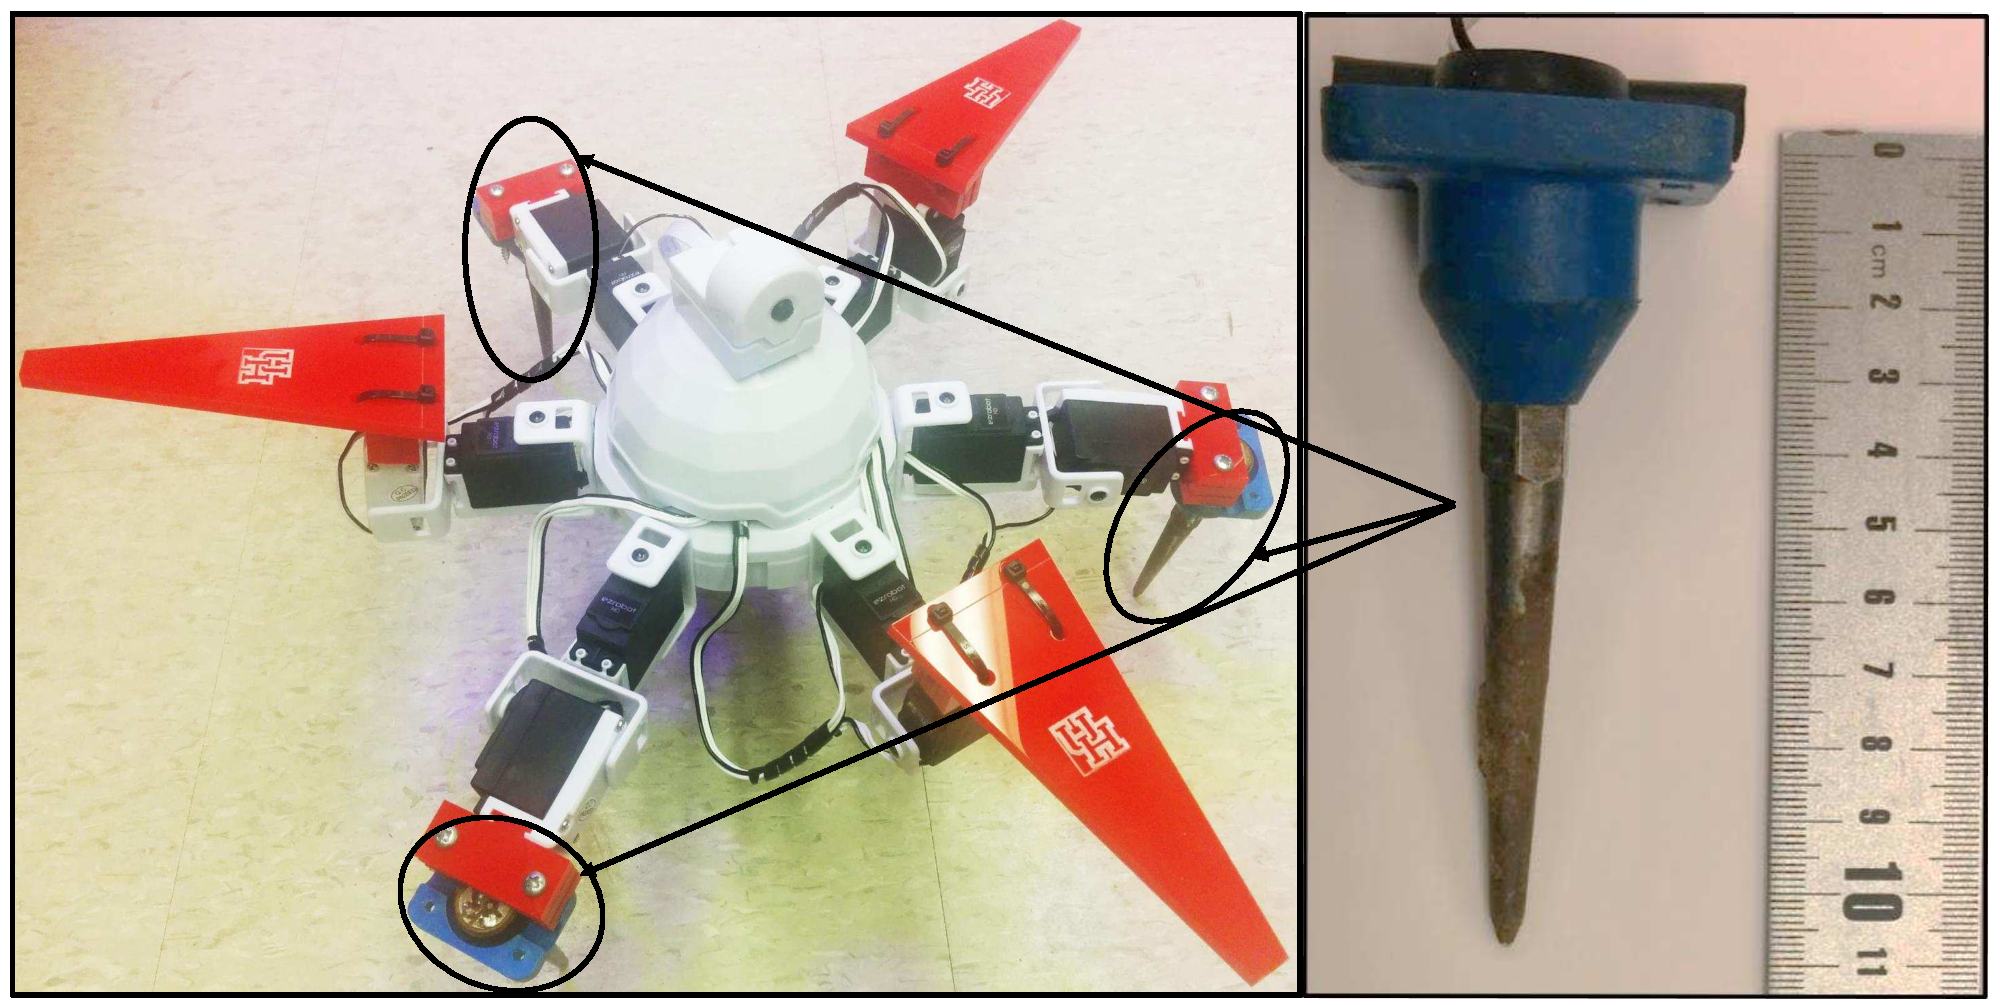
\includegraphics[width=\columnwidth]{ral2016/Hex_overview.pdf}}
	\caption{
		The SeismicSpider is a six-legged mobile robot where geophones replace three legs
		It is drone deployable, can sense and record seismic data, and can move to desired locations, including terrain the SeismicDart cannot access.}
	\label{fig:Hex_overview}
\end{figure}

The SeismicSpider, shown in Fig.~\ref{fig:Hex_overview}, is built from the Six Hexapod kit designed by EZ-Robots.
Each of the six legs is powered by two 15 kg$\cdot$cm lever servos.
Three legs were replaced by three GS-20DM 14 Hz geophones from Geospace Technologies.
The remaining three legs were designed to match the geophone dimensions.

Our initial plan to use three geophones required the spider to raise the three inactive legs while acquiring data.
This lack of support caused excessive strain on the three servo motors responsible for holding the spider upright, introducing unwanted vibration into the system.
Positioning the geophone legs at 20$^\circ$ to normal enhances stability and relieves the excessive stress on the servos.
The three geophones were in series, so with each geophone leg angled inward, superposition replicates the signal from one vertical geophone.

Traditional geophones are mounted in an insulated, shock-resistive enclosure on a spike.
The spikes, varying in length, are inserted into the ground to ensure a firm coupling with the environment.
The design of our SeismicSpider prevents full depth insertion of the 88 mm spikes.

To overcome the coupling issue we are using three geophones per station compared to the typical one.
Our immediate goals were to compare amplitude response to that of a standard single station.	
 
\subsection{Shot gather comparison}
%\subsubsection{Accuracy plot}
%Hexapod move to desired GPS location  (plot accuracy)\\
%\subsubsection{ Shot gather comparison}

A line of twenty-four geophones (GS-20DM 14 Hz) were laid out at one-meter intervals with our inline source seven meters from the nearest geophone.
Beginning from the farthest offset of 31 m we manually aligned the Spider with the corresponding geophone, fired the source, then moved one meter ahead.

%\paragraph{Results}
Data from the shot gather comparison is shown in Fig.~\ref{fig:shotgatherHexpod}.
The response for three geophones in series was 5 dB greater than a single geophone.
The geophone wires proved insufficient to insulate against 60 Hz noise.
Hence the raw data from the traditional setup as well as the SeismicSpider was processed with a (3-50) band-pass filter.
Finally, the SeismicSpider data was attenuated by $-5$dB to level the comparison.

\begin{figure} \centering
	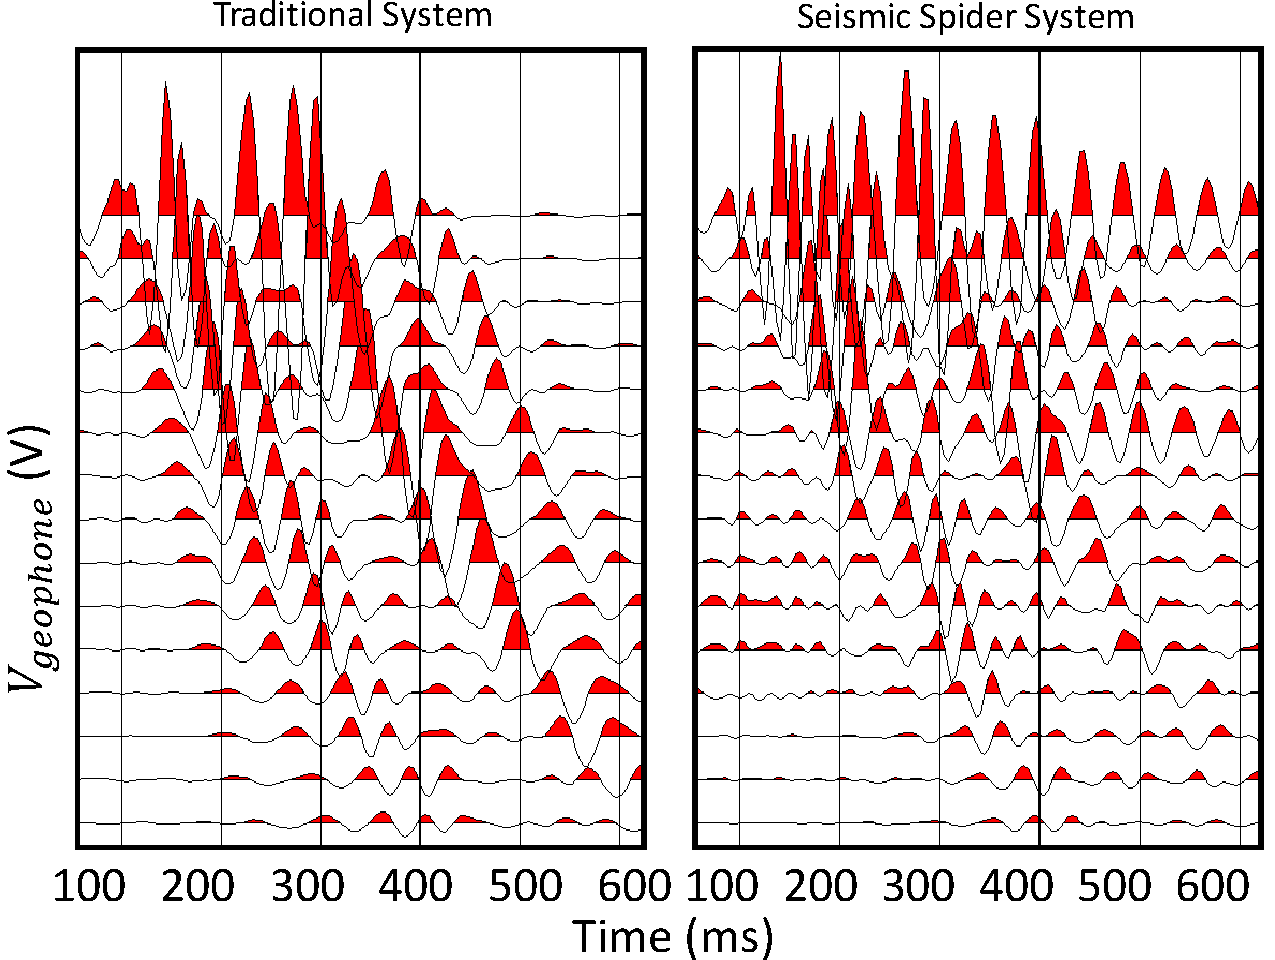
\includegraphics[width=\columnwidth]{ral2016/shotgather_hex.pdf}
	\caption{Shot gather comparison of traditional geophones vs. SeismicSpider.
	\label{fig:shotgatherHexpod}}
\end{figure}

\subsection{Deploying and Retrieving the SeismicSpider}

\begin{figure} \centering
	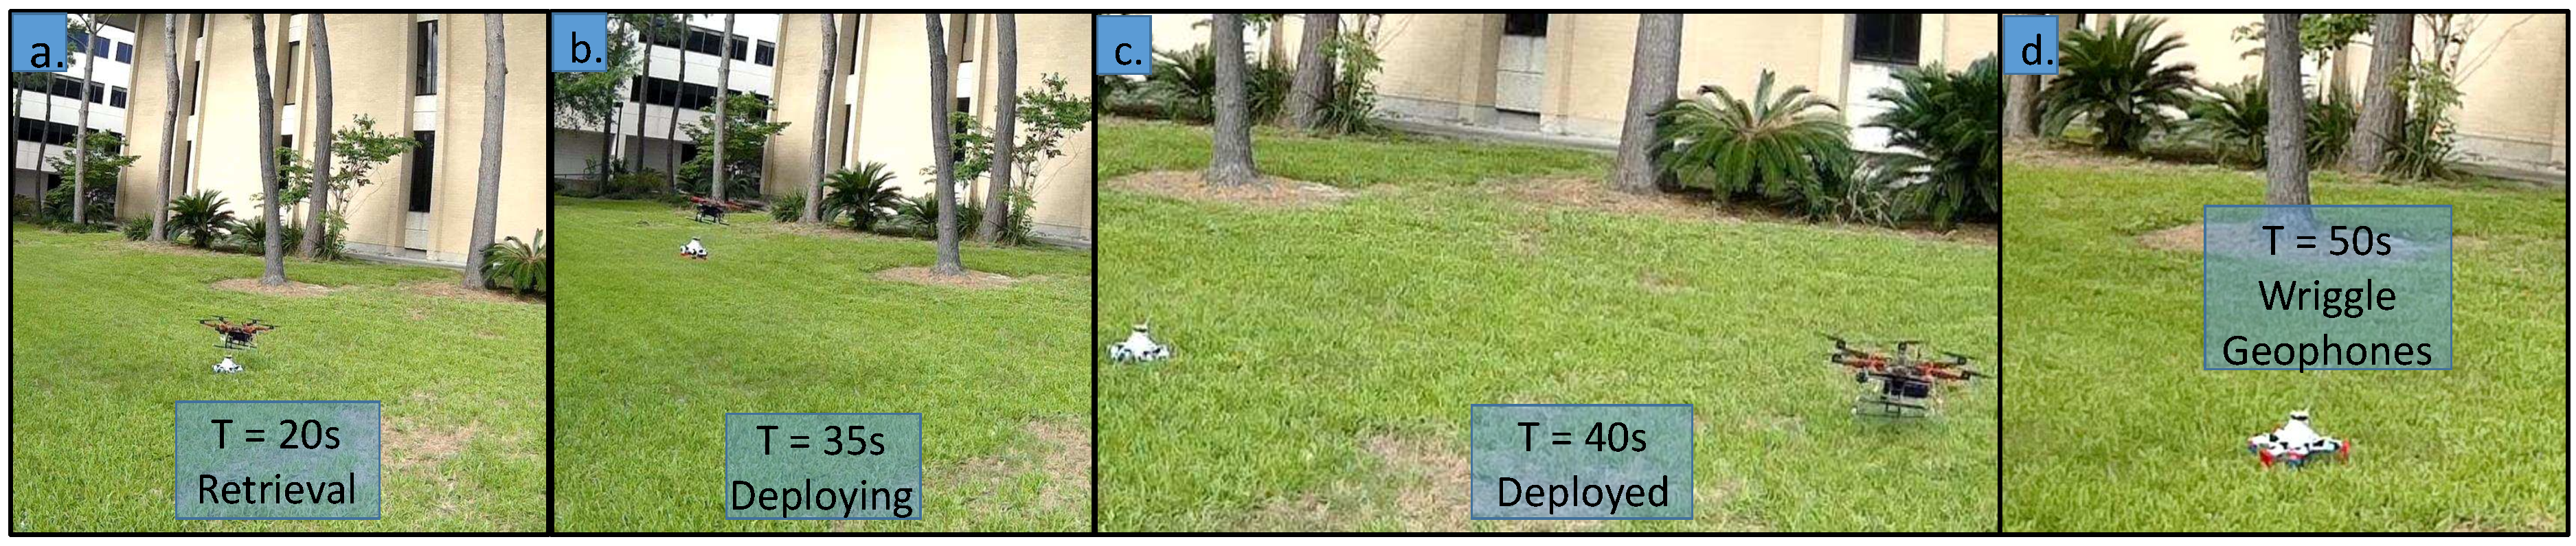
\includegraphics[width=\columnwidth]{ral2016/SeismicSpider_DR.pdf}
	\caption{SeismicSpider retrieval and redeployment. See video attachment.
	\label{fig:SeismicSpiderDR}}
\end{figure}

The UAV's purpose is to deploy sensors at desired GPS waypoint locations.
The SeismicSpider is a mobile robot, but it is substantially slower than the UAV.
The UAV carrying the SeismicSpider flew autonomously to a programmed waypoint.
The deployment mechanism included a hook controlled by a servo attached to the UAV.
The UAV lowered to a waypoint 0.5 m from the ground, then the servo was triggered to unhook the SeismicSpider.
The SeismicSpider was then wirelessly powered on.
The SeismicSpider also has an onboard GPS, enabling it to navigate to desired waypoints.
After walking to the sensing location, the SeismicSpider was programmed to shake its three non-sensing legs to plant its geophone legs into the ground.
Currently, autonomous deployment of sensors is implemented, but the retrieval is piloted.
Combining the mobility of the SeismicSpider with the speed of the UAV enables reaching locations inaccessible by air or impossible to penetrate by SeismicDarts.
Fig.~\ref{fig:SeismicSpiderDR} shows the SeismicSpider being retrieved and then redeployed by a UAV.
